\chapter{Optimal Transport Theory}

To introduce the optimal transport problem please imagine we are asked by a consortium of factories to design a plan for distributing their products among its many customers in such a way that the transportation costs are minimal. \\


We can start the approach of this problem considering the customers as members of the set $X$ and the factories as members of a set $Y$. We want to know which factory $y\in Y$ is going to supply a customer $x\in X$, i.e. we represent such assignation of a factory to a customer as map $y=T(x)\in Y$. Therefore, we can estimate the transportation cost $c(x, T(x))$ of supplying a customer $x$ with a factory $y=T(x)$. 

We see that our problem is reduced to find an assigning map from the set of customers to the set of factories in such a way that the total cost $C(X, Y)=\sum_{x\in X} c(x, T(x))$ is minimal.  
\\
\begin{figure}[H]
	\centering
	\caption{Illustration of the problem of Factories supplying customers.}
	\begin{subfigure}[t]{0.4\textwidth}
		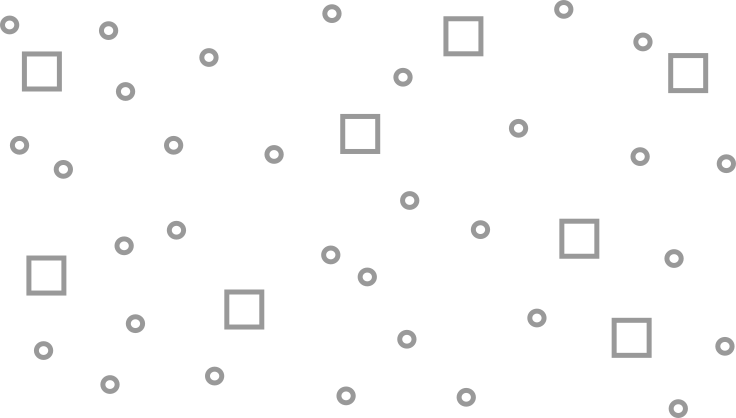
\includegraphics[width=\textwidth]{Factories-Customers.png}
		\caption{Factories represented by squares. customers represented by circles.}
	\end{subfigure}
	\hfil
	\begin{subfigure}[t]{0.4\textwidth}
		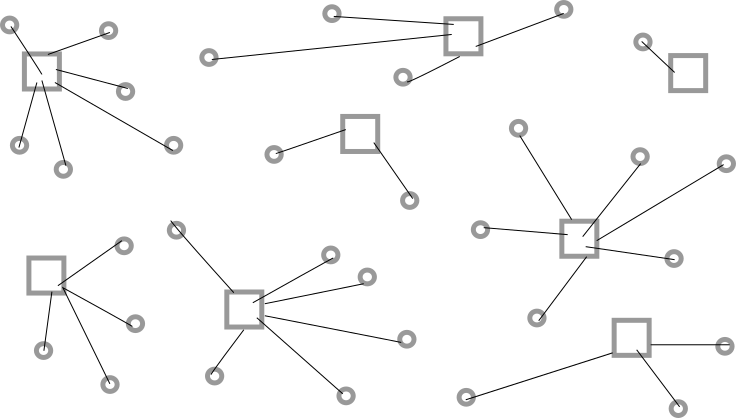
\includegraphics[width=\textwidth]{Factories-Customers-Assignation.png}
		\caption{Factories represented by squares. customers represented by circles. Assignation of a factory to a customer represented by a line.}
	\end{subfigure}	
\end{figure}

Gaspard Monge was a French mathematician who introduced for the very first time the optimal transport problem as \textit{d\'eblais et remblais} in 1781. Monge was interested in finding a map that distributes an amount of sand or soil extracted from the earth or a mine distributed according to a density $f$, onto a new construction whose density of mass is characterized by a density $g$, in such a way the average displacement is minimal. 


We see that Monge presented a more continuous flavor of the transportation problem. In order to avoid ambiguity we make use of modern notation to state a precise idea behind the Monge's problem.

We find convenient the use of measures to describe in a better setting our problem. 
Consider the measures $\mu$ on $X \subset \Real^d$ and $\nu$ on $Y \subset \Real^d$ induced by the nonnegative densities $f$ and $g$ respectively. Moreover, we are only interested in situations 

The space of Borel probability measures on $X$ is denoted by $\PlanSp(X)$. The weak topology on $\PlanSp(X)$ is induced by convergence against bounded continuous test functions on $X$, that is $C_b(X)$.

Given two densities of mass $f$ and $g$, Monge was interested in finding a map $T:\Real^3\rightarrow\Real^3$ pushing the one onto the other,

\begin{equation*}
	\int_A g(y) \dy = \int_{T^{-1}(A)} f(x) \dx  \label{eq: Integral-Borel-MP}
\end{equation*}
For any Borel subset $A\subset\Real^3$. And the transport also should minimize the quantity, 
\begin{equation*}
	\int_{\Real^3} \abs{x-T(x)} f(x)\dx
\end{equation*}
We need to mention that given the context for which the problem was formulated, originally it was binded to $\Real^3$ or $\Real^2$ but we can consider the general case in $\Real^d$. 


Therefore, we need to search for the optimum in the set of measurables maps $T:X \rightarrow Y$ such that the condition \eqref{eq: Integral-Borel-MP} is translated to,

\begin{equation}
	(T_\#\mu)(A)=\mu(T^{-1}(A))
\end{equation}
for every measurable set $A$. In other words, we need $T_\# \mu = \nu$.  In the Euclidean frameworks if we assume $f$, $g$ and $T$ regular enough and $T$ also injective, this equality implies,
\begin{equation}
	g(T(x))\det\parentheses{\D T(x)}=f(x) \label{eq: PDE Monge condition.}
\end{equation} 
\begin{figure}[H]
	\centering
	\caption{Monge problem. Finding a map.}
	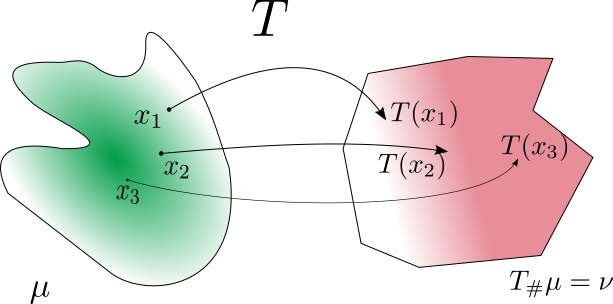
\includegraphics[width=0.4\textwidth]{Monge-Problem-densities.png}
\end{figure}
The equation \eqref{eq: PDE Monge condition.} is nonlinear in $T$ making difficult the analysis of the Monge's Problem. Moreover, the constrain makes this problem hard to handle since it is not close even under weak convergence. 

To appreciate this fact, consider $\mu = \Lebesgue^1\measurerestr[0,1]$ and the hat functions $h_k$ defined as follow,

\begin{equation*}
	h_k(x)=\begin{cases}
		2kx & x\in\brackets{0, \frac{1}{2k}}\\
		2-2kx & x\in \left(\frac{1}{2k}, \frac{1}{k}\right] \\
		0 & \otherwise
	\end{cases}
\end{equation*}
Then take the sequence $f_n:[0,1]\rightarrow [0,1]$,
\begin{equation}
	f_n(x)=\sum_{i=0}^{n-1}h_n\parentheses{x-\frac{i}{n}}
\end{equation}
We see that the sequence satisfies $\Tmeasure{\mu}{f_{n}}=\mu$. It is easy to check that $\mu\parentheses{f_n^{-1}\left(A\right)}=\Lebesgue^1\parentheses{A}$ for every open set $A\in [0,1]$. In the other hand, the sequence converges weakly to $f_n\weakconvergence f=\frac{1}{2}$, which obviously makes $\Tmeasure{\mu}{f}\neq\Lebesgue^1\measurerestr [0,1]$. 


\begin{problem} Given two probability measures $\mu \in \PlanSp\parentheses{X}$ and $\nu \in \PlanSp\parentheses{Y}$ and a cost function $c: X \times Y \rightarrow \braces{0, +\infty}$, the Monge's problem consists in finding a map $T:X\rightarrow Y$
	
\begin{equation}
\inf\braces{\Monge:=\int_X c(x, T(x)) \diff \mu(x): \ \ \Tmeasure{\mu}{T}=\nu }\label{eq: Monge's Problem.}\tag{MP}
\end{equation}
\end{problem}

Monge analyzed geometric properties of the solution to this problem. Although, the problem of the existence stayed open until a Russian mathematician named Leonid Vitaliyevich Kantorovich introduced in the paper \cite{Kantorovich1942} a suitable framework to study its optimality conditions and prove existence of a minimizer. 

If we try to formulate our factories-customer problem through finding an assignation map, we are excluding the situations in which one customer is supplied by two or more factories.

\begin{definition}[Coupling] Let $(X, \mu)$ and $(Y, \nu)$ be two probability spaces. Coupling $\mu$ and $\nu$ means constructing two random variables $\X$ and $\Y$ on some probability space $(\Omega, \mathcal{P})$ such that $\law(\X)=\mu$, $\law(\Y)=\nu$. The couple $(\X,\Y)$ is called a coupling of $(\mu, \nu)$.  
\end{definition}



\begin{definition}[Deterministic Coupling]
A coupling $(\X,\Y)$ is said to be deterministic if there exists a measurable function $T: X \rightarrow Y$ such that $\Y = T(\X)$.
\end{definition}

$\gamma=\Tmeasure{\mu}{\parentheses{\id, T}}=(\mu, \nu)$


\begin{lemma}[Gluing lemma] Let $(\X_i , \mu_i)$, $i = 1, 2, 3$,  be Polish probability spaces. If $(X_1 , X_2)$ is a coupling of $(\mu_1, \mu_2 )$ and $(\Y_2 , Y_3)$ is a coupling of $(\mu_2, \mu_3)$, then it is possible to construct a triple of random variables $(Z_1 , Z_2, Z_3)$ such that $(Z_1, Z_2)$ has the same law as $(X_1 , X_2)$ and $(Z_2, Z_3)$ has the same law as $(Y_2 , Y_3)$.
\end{lemma}


\begin{problem}Given $\mu \in \PlanSp\parentheses{X}$, $\nu \in \PlanSp\parentheses{Y}$, and $c: X\times Y \rightarrow \brackets{0, +\infty}$, we consider the problem
	\begin{equation}
		\inf\braces{\Kantorovich := \int_{X\times Y} c \diff\gamma : \gamma \in \TransPlansSet{\mu}{\nu}}\label{eq: Kantorovich's Problem.}\tag{KP}
	\end{equation}
where $\TransPlansSet{\mu}{\nu}$ is the set of \textit{transport plans}.
\end{problem}



\section{Kantorovich formulation as relaxation}

\begin{theorem}
	Let $X$ and $Y$ be compact metric spaces, $\mu \in \PlanSp(X)$, $\nu \in  \PlanSp$ and
	$c:X\times Y \rightarrow \Real$  a continuous function. Then  \eqref{eq: Kantorovich's Problem.} admits a solution.
\end{theorem} 

\section{Cyclical Monotonicity.}

Consider a similar situation to the factories-customers example, but the consortium has already a fixed distribution plan. They know that transportation costs are high and they want to make them cheaper. Currently, in this expensive plan we choose one factory and we search  


\begin{definition}[c-transform]
	Let $X$ and $Y$ be sets, and $c:X\times Y \rightarrow (-\infty, \infty]$. A function $\psi: X\rightarrow \Realex$ is said to be c-convex if it is not identically to $+\infty$ and there exists $\psi^c: Y \rightarrow \Realex$
	
	\begin{equation}
		\psi^c(y)= \inf_{x\in X} c(x,y)-\psi(x).
	\end{equation}
\end{definition}

\begin{definition}
	Let $X , Y$ be arbitrary sets, and $c:X\times Y \rightarrow (-\infty, \infty]$ be a cost function. A subset $\Gamma \subset X \times Y$ is said to be c-cyclically monotone if, for any $N\in\Naturals$, and any family of points $(x_1, y_1), (x_2, y_2), \dots (x_N, y_N)$ of $\Gamma$, the inequality
	\begin{equation*}
		\sum_{i=1}^{N} c(x_i, y_i) \leq \sum_{i=1}^{N} c(x_i, y_{i+1}) 
	\end{equation*} 
	considering $N+1=1$. 
\end{definition}
Since any permutation $\sigma$ over the set $\braces{1, \dots, N}$ can be written as a product of disjoint cycles, we have that this property satisfies,
\begin{equation}
		\sum_{i=1}^{N} c(x_i, y_i) \leq \sum_{i=1}^{N} c(x_i, y_{\sigma(i)}) 
\end{equation}
\begin{definition}[Support of transport plan.]
	Given a separable metric space $X$, the support of a measure $\gamma$ is defined as the smallest closed set on which $\gamma$ is concentrated,
	\begin{equation}
	\spt(\gamma)\ :=\underset{\small{\begin{array}{c}
		\gamma(X\backslash A)=0\\ A=\bar{A}  \end{array}}}{\bigcap A} 		
	\end{equation} 
\end{definition}
We can fix a point $(x_0, y_0) \in \spt(\gamma)$, then 
\begin{theorem}
	
\end{theorem}

\section{Properties of Optimal plans.}
\section{Wasserstein Spaces. $\WassersteinSp{p}$}